% Created 2024-04-01 Mon 01:05
% Intended LaTeX compiler: pdflatex
\documentclass[a4paper,11pt]{exam}
\usepackage[utf8]{inputenc}
\usepackage[T1]{fontenc}
\usepackage{graphicx}
\usepackage{longtable}
\usepackage{wrapfig}
\usepackage{rotating}
\usepackage[normalem]{ulem}
\usepackage{amsmath}
\usepackage{amssymb}
\usepackage{capt-of}
\usepackage{hyperref}
\usepackage[T1]{fontenc}
\usepackage{titling}
\usepackage{url}
\usepackage{amsmath,amsthm,amssymb}
\usepackage{titling}
\usepackage{url}
\usepackage{amsmath,amsthm,amssymb}
\usepackage{graphicx}
\usepackage{graphics}
\usepackage{listings}
\usepackage[dvipsnames]{xcolor}
\usepackage{tabularx}
\usepackage{ragged2e}
\usepackage{courier}
\usepackage{textcomp}
\usepackage{circuitikz}
\usepackage{tikz}
\usepackage{enumitem}
\usepackage{karnaugh-map}
\usepackage{bytefield}
\usepackage{mathrsfs}
\usepackage{cancel}
\usepackage[linesnumbered,ruled,vlined]{algorithm2e}
\usepackage{hyperref}
\usepackage{environ}
\usepackage{listings}
\usepackage{algorithm}
\usepackage{algpseudocode}
\lstset{breaklines=true, basicstyle=\ttfamily\tiny, frame=single, escapeinside={(*@}{@*)}}
\usepackage[margin=0.75in]{geometry}
\author{Miguel Gomez U1318856}
\date{2024-04-01 01:05:53}
\title{Homework Assignment \# 3}
\hypersetup{
 pdfauthor={Miguel Gomez U1318856},
 pdftitle={Homework Assignment \# 3},
 pdfkeywords={},
 pdfsubject={},
 pdfcreator={Emacs 28.2 (Org mode 9.4.6)}, 
 pdflang={English}}
\begin{document}

\maketitle
\tableofcontents

\newpage

\section{HW3 - Problem 1}
\label{sec:org720b577}
design an elliptic curve crypto-cipher over a Galois field of the type \(\mathbb{F}_{2^k}\).  Implement the key generation, encryption and decryption modules in Singular, and demonstrate the correct simulation.
\subsection{a) what are \(\alpha^4 , \alpha^5 , \alpha^6\) when reduced (mod \(P(\alpha)\))}
\label{sec:org7f91e5e}
Consider the finite field \(\mathbb{F}_{2^k} \equiv \mathbb{F}_{2}[x]\) (mod \(P(x)\)) where \(P(x) = x^3 + x^2 + 1\). Let \(\alpha\) be a root of \(P(x)\), i.e. \(P(\alpha) = 0\). Note that \(P(x)\) is indeed a primitive polynomial. Using Singular, enumerate the field elements \(F_8 = {0, \alpha^7 = 1, \alpha, \alpha^2, \alpha^3 = \alpha^2 + 1, \alpha^4 =?, . . . , \alpha^6 =?}\). In other words, what are \(\alpha^4 , \alpha^5 , \alpha^6\) when reduced (mod \(P(\alpha)\))?

\begin{verbatim}
start=$(date +%s.%N)
Singular ./sing/point_enumeration.sing | grep -v -e \
				      "Mathematik\|^ \|//\|\*\* loaded\|\*\* library"
end=$(date +%s.%N)
echo "Execution Time: $(echo "$end - $start" | bc) seconds"
\end{verbatim}


\[
\subsubsection{output of point-enumeration.sing results}
\begin{lstlisting}[language=Singular]
================================
when x = 0
poly f is:
y2+1
poly f factorizes as follows:
[1]:
[2]:
================================
when x = A^0, : x = 1
P1(x,y) = (1,y2+(A2))
================================
when x = A^1, : x = (A)
P1(x,y) = ((A),1)
P2(x,y) = ((A),y+(A+1))
================================
when x = A^2, : x = (A2)
P1(x,y) = ((A2),(A))
P2(x,y) = ((A2),y+(A2+A))
================================
when x = A^3, : x = (A2+1)
P1(x,y) = ((A2+1),(A+1))
P2(x,y) = ((A2+1),y+(A2+A))
================================
when x = A^4, : x = (A2+A+1)
P1(x,y) = ((A2+A+1),(A))
P2(x,y) = ((A2+A+1),y+(A2+1))
================================
when x = A^5, : x = (A+1)
P1(x,y) = ((A+1),0)
P2(x,y) = ((A+1),y+(A+1))
================================
when x = A^6, : x = (A2+A)
P1(x,y) = ((A2+A),1)
P2(x,y) = ((A2+A),y+(A2+A+1))
================================
when x = A^7, : x = 1
P1(x,y) = (1,y2+(A2))
================================
Auf Wiedersehen.
Execution Time: .044122341 seconds
\end{lstlisting}
\]


As can be seen in the output below, \(\alpha^4,\ \alpha^5,\ \alpha^6\) are as follows:

\begin{align*}
\alpha^4 &= \alpha^2+\alpha+1\\
\alpha^5 &= \alpha+1\\
\alpha^6 &= \alpha^2+\alpha
\end{align*}


\subsection{b)  Enumerate all the points on the curve}
\label{sec:orgdee9dbb}

\begin{verbatim}
start=$(date +%s.%N)
Singular ./sing/point_gen.sing  | grep -v -e \
				      "Mathematik\|^ \|//\|\*\* loaded\|\*\* library"
end=$(date +%s.%N)
echo "Execution Time: $(echo "$end - $start" | bc) seconds"
\end{verbatim}


\[
\subsubsection{output of point\_gen.sing results}
\begin{lstlisting}[language=Singular]
P = ((A2+1), (A+1))
Calling doubleP on P
received/ 2P:
2P = ((A2), (A2+A))
3P = ((A2+A), (A2+A+1))
4P = ((A), (A+1))
5P = ((A+1), 0)
6P = ((A2+A+1), (A2+1))
7P = (0, 1)
8P = ((A2+A+1), (A))
9P = ((A+1), (A+1))
10P = ((A), 1)
11P = ((A2+A), 1)
12P = ((A2), (A))
13P = ((A2+1), (A2+A))
14P = (0, 0)
15P = ((A), (A2+A+1))
16P = ((A2+1), (A2+A))
Auf Wiedersehen.
Execution Time: .043611095 seconds
\end{lstlisting}
\]


Shown above is the enumeration of the points and below they are added with nicer formatting.
\begin{align*}
  P &= (\alpha^2+1, \alpha+1)\\
  2P &= (\alpha^2, \alpha^2+\alpha)\\
  3P &= (\alpha^2+\alpha, \alpha^2+\alpha+1)\\
  4P &= (\alpha, \alpha+1)\\
  5P &= (\alpha+1, 0)\\
  6P &= (\alpha^2+\alpha+1, \alpha^2+1)\\
  7P &= (0, 1)\\
  8P &= (\alpha^2+\alpha+1, \alpha)\\
  9P &= (\alpha+1, \alpha+1)\\
  10P &= (\alpha, 1)\\
  11P &= (\alpha^2+\alpha, 1)\\
  12P &= (\alpha^2, \alpha)\\
  13P &= (\alpha^2+1, \alpha^2+\alpha)\\
  14P &= (0, 0)
 \end{align*}

\subsection{c)  Identify a point \(P(x, y)\) that acts as a primitive element}
\label{sec:org3207b7b}

This result above provided by the Singular procedure proves that we can generate the points on the curve as well as proving that our starting point below is a generator.

\begin{align*}
P &= (\alpha^3,\alpha^5) = (\alpha^2 + 1, \alpha + 1)
\end{align*}


\subsection{d) Is its inverse point \(P^{-1}\) also a generator of G?}
\label{sec:orgfe13506}
Let a point \(P(x1 , y1)\) be a generator of \(G = \left<E, +\right>\). Is its inverse point \(P^{-1}\) also a generator of \(G\)? If yes, then prove it. Otherwise, give a counterexample.
\newline
\newline
If we take the expression for the primitive inverse point and apply it to our point \(P\), we can then run the same algorithm for generation of points on the inverse to see what we get.

\begin{align*}
 P &= (x_1,y_1)\\
 P^{-1} &= (x_1,x_1+y_1)\\
 P &= (\alpha^2+1, \alpha+1)\\
 P^{-1} &= (\alpha^2+1, \alpha^2+\alpha)
\end{align*}

\begin{verbatim}
start=$(date +%s.%N)
Singular ./sing/point_inversion.sing  | grep -v -e \
				      "Mathematik\|^ \|//\|\*\* loaded\|\*\* library"
end=$(date +%s.%N)
echo "Execution Time: $(echo "$end - $start" | bc) seconds"
\end{verbatim}


\[
\subsubsection{output of inversion results}
\begin{lstlisting}[language=Singular]
Normal  generator P     = ((A2+1), (A+1))
Inverse generator P^-1  = ((A2+1), (A2+A))
Printing the inverse generated points:
printing 1P:
((A2+1), (A2+A))
printing 2P:
((A2), (A))
printing 3P:
((A2+A), 1)
printing 4P:
((A), 1)
printing 5P:
((A+1), (A+1))
printing 6P:
((A2+A+1), (A))
printing 7P:
(0, 1)
printing 8P:
((A2+A+1), (A2+1))
printing 9P:
((A+1), 0)
printing 10P:
((A), (A+1))
printing 11P:
((A2+A), (A2+A+1))
printing 12P:
((A2), (A2+A))
printing 13P:
((A2+1), (A+1))
printing 14P:
(0, 0)
Auf Wiedersehen.
Execution Time: .043077703 seconds
\end{lstlisting}
\]



\noindent
Looks like the results show that we can indeed perform point generation using the inverse point. Here is the set of points generated by the inverse point. 
\begin{align*}
  P^{-1} &= (\alpha^2+1, \alpha^2+\alpha)\\
  2P^{-1} &= (\alpha^2, \alpha)\\
  3P^{-1} &= (\alpha^2+\alpha, 1)\\
  4P^{-1} &= (\alpha, 1)\\
  5P^{-1} &= (\alpha+1, \alpha+1)\\
  6P^{-1} &= (\alpha^2+\alpha+1, \alpha)\\
  7P^{-1} &= (0, 1)\\
  8P^{-1} &= (\alpha^2+\alpha+1, \alpha^2+1)\\
  9P^{-1} &= (\alpha+1, 0)\\
  10P^{-1} &= (\alpha, \alpha+1)\\
  11P^{-1} &= (\alpha^2+\alpha, \alpha^2+\alpha+1)\\
  12P^{-1} &= (\alpha^2, \alpha^2+\alpha)\\
  13P^{-1} &= (\alpha^2+1, \alpha+1)\\
  14P^{-1} &= (0, 0)
 \end{align*}
 \noindent
Notice that this list is the same as those generated by \(P\) but in reverse. As in point \(P\) is the same as point \(13P^{-1}\), point \(2P\) is point \(12P^{-1}\), and so on.

\subsection{e) simulate El Gamal encipherment}
\label{sec:org3c642a1}
Using the solutions to the above questions, you will now simulate El Gamal encipherment over the above elliptic curve.

\subsubsection{selecting parameters for encryption}
\label{sec:orgba17ca0}
Based on Fig.1, which is reproduced from our slides, select \(e_1\) as a generator of \(G = \left<E, +\right>\). Select integers \(d\), \(r\), such that \(d \ne r\).

\begin{center}
\begin{figure}[h]
    \centering
    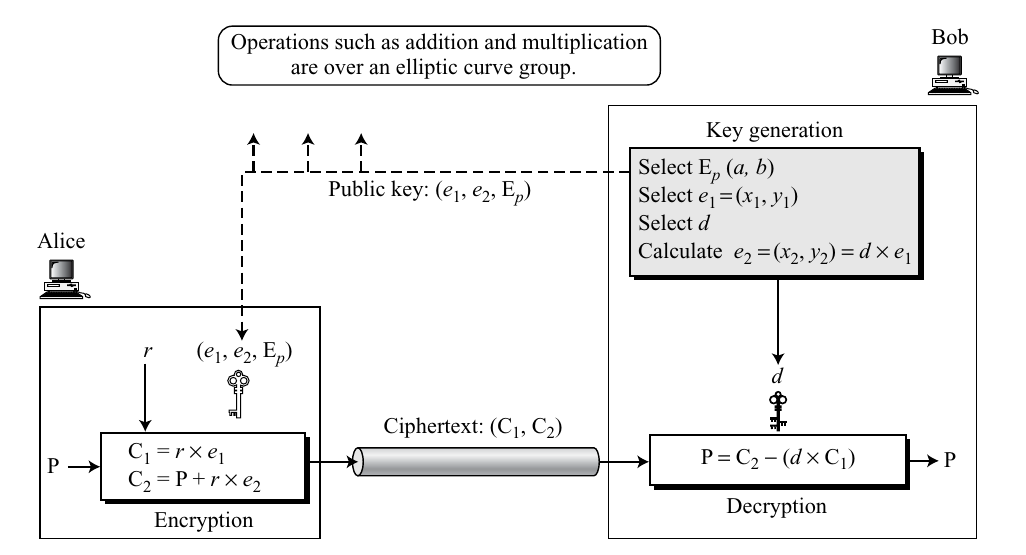
\includegraphics[width=16cm]{./images/fig1_hw3.png}
    \caption{El Gamal over ECC}
    \label{fig:fig1_hw3}
  \end{figure}
\end{center}

\subsubsection{Selecting plain-text}
\label{sec:org791f081}
Select the plaintext \(P\) as a point on the elliptic curve. Compute \(C_1\) , \(C_2\) to demonstrate encryption. \textcolor{red}{NOTE*}[Avoid \(P = (0, 1)\), as it is a trivial point on our non-supersingular curves over \(\mathbb{F}_{2^k}\) ].
I will choose a \(d\) to be some number and calculate the \(e_2\) value. After that, we will calculate the \(c_1\) and \(c_2\) with the \(r\) chosen. Once we are set, we can use the procedures in my ecclib library to process the data. We can map letters up to the 14th letter in the alphabet, and see how that goes.

\subsubsection{process}
\label{sec:orgd42152d}
\noindent
As seen in the slides, we can follow the following process to get the encryption done. we select \(e_1\) first, then proceed as Bob.
\begin{align*}
\text{Bob} : &\text{Select }e_1\\
&\text{Select }d\\
\text{Calculate: }e2 &= d\cdot e_1\\
\text{Bob }(e1,e2,E_p) &\xrightarrow{}\text{Alice}\\
\text{Alice} : C_1 &= r\cdot e_1\\
C_2 &= P + r\cdot e_2\\
\text{Alice }(C_1, C_2) &\xrightarrow{}\text{Bob}
\end{align*}
\subsubsection{encrypter}
\label{sec:orga2b26b3}
\begin{align*}
\text{Alice} : C_1 &= r\cdot e_1\\
C_2 &= P + r\cdot e_2\\
\text{Alice }(C_1, C_2) &\xrightarrow{}\text{Bob}
\end{align*}

\noindent
The encrypter expects that the \(e_1\) and \(e_2\) values are already known as well as the curve we use for encoding points. Knowing this, we can first set up the parameters needed for this calculation and then proceed with calculating the \(C_1\) and \(C_2\) values. This process is shown above and in the output of encrypter.sing below:

\begin{verbatim}
cat ./sing/encrypt.sing
\end{verbatim}


\[
\subsubsection{encrypt.sing file}
\begin{lstlisting}[language=Singular]
LIB "/home/speedy/repos/coursework/hw_crypto/lib/ecclib.lib";

// Declare the ring over GF(8), with 2 variables, x and y
ring r = (2, A), (y, x), lp;
// This is the primitive polynomial given to us as a specification
// Here X = \alpha
minpoly = A^3 + A^2 + 1;

// This is the non-singular elliptic curve also given to us as the spec Weirstrauss form E(A^2, 1)
poly E = y^2 + x*y + x^3 + A^2*x^2 + 1;

// number = element in the field
int D, R;
number x1, y1;
list C1, C2;
list e1, e2;
list P_text;
R = 3;
D = 2;
string P = "A";

// normal generator point below
x1 = A^3;
y1 = A^5;
e1 = x1, y1;
list points = genPoints(e1);
printf("Normal  generator P = (%s, %s)", e1[1], e1[2]);


printf("e1: (%s, %s)",e1[1], e1[2]);
e2 = doubleP(e1);
int e2_ind = getIndex(points,e2);
printf("e2: (%s, %s)",e2[1], e2[2]);
printf("e2 Index: %s",e2_ind);
list point_at_e2_index = getPoint(points, e2_ind);
printf("points[e2_index]: (%s,%s)",point_at_e2_index[1],point_at_e2_index[2]);
"(e1,e2,Ep) -> Alice";
"alice calcs C1 and C2";
printf("C1 = r*e1 = %s*e1 =", R);
C1 = PaddQ(doubleP(e1),e1);
printf("C1: (%s, %s)",C1[1], C1[2]);
printf("plain text P_tex:%s corresponds to point:%s",P,CharToNum(P)+1);
P_text = e1; // point1 e1 = A
C2 = PaddQ(PaddQ(doubleP(e2),e2),P_text);
printf("C2 = P_text + %s*e2 = (%s, %s)",R, C2[1], C2[2]);
"(C1,C2) -> Bob";
printf("C1 (%s, %s) : C2 (%s, %s)", C1[1], C1[2], C2[1], C2[2]);
quit;
\end{lstlisting}
\]


\subsubsection{decrypter}
\label{sec:org321329e}
\begin{align*}
\text{Bob} : P = C_2 - d\cdot C_1\\
\end{align*}

\noindent
The decrypting happens on Bobs end and also requires the same setup. So here we set up the work needed to get \(C_1\) and \(C_2\) as we did before, but now calculate the \(P\) value using that pair of points calculated by Alice. This process was already covered above but needed here and only the last calculation is relevant to the decryption:

\begin{verbatim}
cat ./sing/decrypt.sing
\end{verbatim}


\[
\subsubsection{output of decrypt.sing results}
\begin{lstlisting}[language=Singular]
LIB "/home/speedy/repos/coursework/hw_crypto/lib/ecclib.lib";

// Declare the ring over GF(8), with 2 variables, x and y
ring r = (2, A), (y, x), lp;
// This is the primitive polynomial given to us as a specification
// Here X = \alpha
minpoly = A^3 + A^2 + 1;

// This is the non-singular elliptic curve also given to us as the spec Weirstrauss form E(A^2, 1)
poly E = y^2 + x*y + x^3 + A^2*x^2 + 1;

// number = element in the field
int D, R;
number x1, y1;
list C1, C2;
list e1, e2;
list P_text;
R = 3;
D = 2;
string P = "A";

// normal generator point below
x1 = A^3;
y1 = A^5;
e1 = x1, y1;
list points = genPoints(e1);
e2 = doubleP(e1);
int e2_ind = getIndex(points,e2);
list point_at_e2_index = getPoint(points, e2_ind);
C1 = PaddQ(doubleP(e1),e1);
P_text = e1; // point1 e1 = A
C2 = PaddQ(PaddQ(doubleP(e2),e2),P_text);
// rest of the algo for the decrypting
 
"(C1,C2) -> Bob";
"P = C2 - d*C1";
"P = C2 + (d*C1)^-1";
list d_c1 = PaddQ(doubleP(C1),C1);
int inv_index = getInverseIndex(points, d_c1);
int C2_index = getIndex(points, C2);
printf("= (%s, %s) + (%s, %s)^-1 = P_%s + P_%s = P_%s = P_%s", C2[1], C2[2], d_c1[1], d_c1[2], C2_index, (14 - inv_index)-1, (C2_index + (14 - inv_index)-1 ), (C2_index + (14 - inv_index)-1 )%14);
int plain_text_index = (C2_index + (14 - inv_index)-1 )%14;
"now that we have the index, we can convert back to plain text with NumToChar function we made:";
printf("point P_%s corresponds to %s", plain_text_index, NumToChar(plain_text_index - 1));
quit;
\end{lstlisting}
\]




\subsubsection{Demonstrate decryption by re-obtaining the plaintext \(P\)}
\label{sec:orgd6ac3f6}
Using \(d = 2\) and \(r = 3\):
\begin{align*}
e_1 &= P_1 = (\alpha^3, \alpha^5)\\
e_2 &= d\cdot e_1 = 2\cdot e_1\\
e_2 &= 2\cdot P_1 = P_2 = (\alpha^2, \alpha^2+\alpha)
\end{align*}
Encrypting: \(P = A\) and we can map this letter to the first point \(P_1\). If we could continue for the other letters, we would have to stor at 14 since we only have that many unique points. Meaning we can use up to N in the alphabet.
\begin{align}
A &= P_{1}\\
B &= P_{2}\\
C &= P_{3}\\
D &= P_{4}\\
E &= P_{5}\\
F &= P_{6}\\
G &= P_{7}\\
H &= P_{8}\\
I &= P_{9}\\
J &= P_{10}\\
K &= P_{11}\\
L &= P_{12}\\
M &= P_{13}\\
N &= P_{14}
\end{align}
Getting started, we calculate the \(C_1\) and \(C_2\) that we need to send back to Bob and include our point encoded letter \(A\). 
\begin{align*}
C_1 &= r\cdot e_1 = 3\cdot P_1 = P_3\\
    &= (\alpha^2+\alpha, \alpha^2+\alpha+1)\\
C_2 &= P + r\cdot e_2 = P_1 + 3\cdot P_2 = P_1 + P_6 = P_7\\
    &= (0, 1)
\end{align*}
Seeing it here, any letter we come up with would just have to have \(P_6\) added to it if we keep the \(r\) the same.


Decrypting \(A\):
\begin{align*}
\text{Bob} : P &= C_2 - d\cdot C_1\\
&= P_7 - P_6 = P_7 + P_8 = P_{15}\mod{14} = P_1\\
&= (\alpha^2+1, \alpha+1)
\end{align*}
Say we had a message like the text "JACK", we can encrypt each letter with the corresponding point.
\begin{align*}
\text{JACK} &\xrightarrow{MAP}P_{10}P_{1}P_{3}P_{11}\\
P_{10} &\xrightarrow{ENC} P_{16}\mod{14} = P_{2}\\
P_{1} &\xrightarrow{ENC} P_{7}\mod{14} = P_{7}\\
P_{3} &\xrightarrow{ENC} P_{9}\mod{14} = P_{9}\\
P_{11} &\xrightarrow{ENC} P_{17}\mod{14} = P_{3}\\
 &\xrightarrow{} P_{2}P_{7}P_{9}P_{3}\\
 &\xrightarrow{} BGIC
\end{align*}

\begin{align*}
P_{2}P_{7}P_{9}P_{3}&\xrightarrow{DEC} \\
P_{2} - P_6 &= P_{2} + P_{8} \xrightarrow{DEC} P_{10}\mod{14} = P_{10}\\
P_{7} - P_6 &= P_{7} + P_{8} \xrightarrow{DEC} P_{15}\mod{14} = P_{1}\\
P_{9} - P_6 &= P_{9} + P_{8} \xrightarrow{DEC} P_{17}\mod{14} = P_{3}\\
P_{3} - P_6 &= P_{3} + P_{8} \xrightarrow{DEC} P_{11}\mod{14} = P_{11}\\
P_{10}P_{1}P_{3}P_{11}&\xrightarrow{MAP}\text{JACK}
 \end{align*}
Obviously, this is not secure. We would really want to have a large number of points that we can use for mapping and include more chars. enough to hold all chars in the Unicode standard or something, and also change up the r value used in the calculation along the way. This just made it simpler for us in the displaying of the algo. Below is the output of the files covered above. Instead of running for the whole word like I wanted, I ran into some snags with indices as the way the list is populated in Singular is non trivial. It stores values linearly, so the indices are not a 1 to 1 mapping. I created some helper procedures that are shown in ecclib.lib, and the location of this must be updated in the files I submitted. Unfortunately, Singular is not great with library linking for lib inclusions like C. 

\begin{verbatim}
start=$(date +%s.%N)
Singular ./sing/encrypt.sing | grep -v -e \
				     "Mathematik\|^ \|//\|\*\* loaded\|\*\* library"
end=$(date +%s.%N)
echo "Execution Time: $(echo "$end - $start" | bc) seconds"
\end{verbatim}


\[
\subsubsection{output of encrypt.sing}
\begin{lstlisting}[language=Singular]
Normal  generator P = ((A2+1), (A+1))
e1: ((A2+1), (A+1))
e2: ((A2), (A2+A))
e2 Index: 2
points[e2_index]: ((A2),(A2+A))
(e1,e2,Ep) -> Alice
alice calcs C1 and C2
C1 = r*e1 = 3*e1 =
C1: ((A2+A), (A2+A+1))
plain text P_tex:A corresponds to point:1
C2 = P_text + 3*e2 = (0, 1)
(C1,C2) -> Bob
C1 ((A2+A), (A2+A+1)) : C2 (0, 1)
Auf Wiedersehen.
Execution Time: .042499921 seconds
\end{lstlisting}
\]



\begin{verbatim}
start=$(date +%s.%N)
echo "#+end_example"
Singular ./sing/decrypt.sing | grep -v -e \
				    "Mathematik\|^ \|//\|\*\* loaded\|\*\* library"
echo "#+end_example"
end=$(date +%s.%N)
echo "Execution Time: $(echo "$end - $start" | bc) seconds"
\end{verbatim}


\[
\subsubsection{output of decrypt.sing}
\begin{lstlisting}[language=Singular]
(C1,C2) -> Bob
P = C2 - d*C1
P = C2 + (d*C1)^-1
= (0, 1) + ((A+1), (A+1))^-1 = P_7 + P_8 = P_15 = P_1
now that we have the index, we can convert back to plain text with NumToChar function we made:
point P_1 corresponds to A
Auf Wiedersehen.
Execution Time: .042007079 seconds
\end{lstlisting}
\]

\noindent
To get this done, I implemented a few things in my own ecc library that I can use in the future. Included in this library are the following procedures:
\begin{center}
\begin{tabular}{|c|c|c|c|}
\hline
Procedure Name  & args &  returns  & working \\
\hline
doubleP(a) & Point as list of $x,y$  & Point as list of $x,y$ & \checkmark \\
\hline
PaddQ(a,b) & Points P,Q as list of $x,y$ & Point as list of $x,y$ & \checkmark \\
\hline
genPoints(a) & Point as list of $x,y$ & List of points as a list of lists  & \checkmark \\
\hline
getPoint(a,b) & list of Points&&\\
& an index & Point as list of $x,y$ & \checkmark \\
\hline
getIndex(a,b) & list of Points&&\\
&  target Point as list of $x,y$ & Index of point  & \checkmark \\
\hline
getInverseIndex(a,b) & list of Points&&\\
&  target Point as list of $x,y$ & Point as list of $x,y$  & \checkmark \\
\hline
NumToChar(a)&point number & char of letter & \checkmark\\
\hline
CharToNum(a)& string of letter & point number & \checkmark\\
\hline
\end{tabular}
\end{center}

\noindent
I did not include the full file here or the algos, but these can be referenced in ecclib.lib. There are some other procedures that I am working on that will be used for full message encryption and decryption later on when I get around to fixing the problems. 
\subsection{f) Notes:}
\label{sec:org6859796}
Note: Implement the above in Singular. Please make use of “procedures” in Singular to make your code Modular. Print out the relevant parts of your computation to make it easier for me and  the grader  to grade it when I run your code.  Attach a README to help me understand how to run your code.  Also,  in a PDF file, please  describe  (briefly)  which points you are using as generators, what are your keys \(e_1\) , \(e_2\) , \(d\), \(r\) and the corresponding \(P\), \(C_1\), \(C_2\) values. 

\newline
\noindent
Description of params for easy lookup:

\begin{align*}
  d &= 2\\
  r &= 3\\
e_1 &= (\alpha^3,\alpha^5)\\
e_2 &= (\alpha^2,\alpha^2 + \alpha)\\
  P &= (\alpha^2 + 1,\alpha + 1)\\
C_1 &= (\alpha^2 + \alpha,\alpha^2 + \alpha + 1)\\
C_2 &= (0,1)\\
\end{align*}

\noindent
The description technically lies within this file as the output of the code is inline as well as the commands run to get them. All of them can be copy pasted into the terminal and the same results should be present as long as the lib inclusion is set up for the environment the grader is using. Please reach out and let me know if there are problems with the execution, and I can help setting up your environment correctly. 

\subsection{g) Permissions for using skeleton provided}
\label{sec:orge8e1156}
It goes without saying: feel free to borrow inspirations from the Singular files I used to give you a demo of ECC El Gamal in class; those Singular files are uploaded on Canvas: ecc-f8-example.sing.



\section{Problem 2}
\label{sec:orgfa62b9a}
In this question, you will design a digital logic circuit that performs point doubling \(R = 2P\)  (not point addition!) over elliptic curves using the projective coordinate system. You will first design (or re-use from HW 2) a multiplier circuit, use it as a building block to perform doubling. You will implement your design in Verilog or VHDL, and demonstrate that point addition is being performed correctly.

\subsection{a) Defining field and terms}
\label{sec:org9013fed}
We will use the same finite field as in the previous question: F8 ≡ F2 [x] (mod P(x) =x3 + x2 + 1) with P(α) = 0. Denote the degree of P(x) as k; of course, here k = 3.

\subsection{b) Design multiplier}
\label{sec:org84c0fec}
Design a k = 3 bit finite field multiplier that takes A = \{a2, a1 , a0 \} and B = \{b2 , b1 , b0 \} as 3-bit inputs, and produces Z = \{z2 , z1 , z0\} as a 3-bit output. Note that we will have:

\begin{align*}
A &= a_0 + a_1 \alpha + a_2\alpha^2\\
B &= b_0 + b_1 \alpha + b_2\alpha^2\\
Z &= z_0 + z_1 \alpha + z_2\alpha^2
\end{align*}

\noindent
Such that \(Z = A \cdot B\) mod \(P(\alpha))\). Of course, you have already designed 2 multipliers in the last HW (Mastrovito and Montgomery). Just pick whichever one you like. Also, please double check that the primitive polynomial that you used in the design of HW 2 was indeed \(P(x) = x^3 + x^2 + 1\).


\noindent 
I prevously attempted implementation of the algorithm for the mastrovito multiplier over \(\mathbb{F}_8\) but was unable to get it working as intended. Here I have tried setting up the professors implementation of the multiplier which is closer to the one that I made with my GFMult in HW2.

\begin{verbatim}
cat ./verilog/MM.v
\end{verbatim}


\[
\subsubsection{Verilog code for mastro mult}
\begin{lstlisting}[language=verilog]
module MM (
	   input wire [2:0] A,
	   input wire [2:0] B,
	   input wire	   clk,
	   input wire	   reset,
	   output reg [2:0] Z
	   );

always@(*)
  begin
     Z[0] = (A[0] & B[0]) ^ (A[1] & B[2]) ^ (A[2] & B[1]) ^ (A[2] & B[2]);
     Z[1] = (A[0] & B[1]) ^ (A[1] & B[0]) ^ (A[2] & B[2]);
     Z[2] = (A[0] & B[2]) ^ (A[1] & B[2]) ^ (A[2] & B[0]) ^ (A[2] & B[2]) ^ (A[1] & B[1]) ^ (A[2] & B[1]);
  
  end 
endmodule // MM
\end{lstlisting}
\]





\subsection{c) Implementation in Verilog}
\label{sec:orgf075870}
Implement the design in Verilog/VHDL (GFMult(A, B, Z) module) and demonstrate/simulate using a testbench the following input-output combinations:

\noindent
Here is the GFMULT module in verilog:

\begin{verbatim}
cat ./verilog/GFMult.v
\end{verbatim}


\[
\subsubsection{GFMULT.v file}
\begin{lstlisting}[language=verilog]
module GFMult (
	       input wire	 clk, // Clock input
	       input wire	 reset, // Asynchronous reset input
	       input wire [2:0]	 A, // 3-bit input of the Multiplier
	       input wire [2:0]	 B, // 3-bit input of the Multiplier
	       output reg [2:0] Z // 3-bit output of the Multiplier
	       
	       );
   wire				 s0, s1, s2, s3, s4;

   assign s0 = A[0]&B[0];
   assign s1 = A[1]&B[0] ^ A[0]&B[1];
   assign s2 = A[2]&B[0] ^ A[1]&B[1] ^ A[0]&B[2];
   assign s3 = A[2]&B[1] ^ A[1]&B[2];
   assign s4 = A[2]&B[2];
   
always@(posedge reset, negedge clk) begin
   if(reset) begin
      Z <= 3'b0;
   end   
   else begin
      Z[0] <= (s0 ^ s3 ^ s4);
      Z[1] <= (s1 ^ s4);
      Z[2] <= (s2 ^ s3 ^ s4);      
   end 
end
   
endmodule
\end{lstlisting}
\]

\noindent
And here is the MM module implementation in verilog as well. This using the version by Prof Kalla since I was unable to get mine functioning as I wanted:

\begin{verbatim}
cat ./verilog/MM.v
\end{verbatim}


\[
\subsubsection{MM.v file}
\begin{lstlisting}[language=verilog]
module MM (
	   input wire [2:0] A,
	   input wire [2:0] B,
	   input wire	   clk,
	   input wire	   reset,
	   output reg [2:0] Z
	   );

always@(*)
  begin
     Z[0] = (A[0] & B[0]) ^ (A[1] & B[2]) ^ (A[2] & B[1]) ^ (A[2] & B[2]);
     Z[1] = (A[0] & B[1]) ^ (A[1] & B[0]) ^ (A[2] & B[2]);
     Z[2] = (A[0] & B[2]) ^ (A[1] & B[2]) ^ (A[2] & B[0]) ^ (A[2] & B[2]) ^ (A[1] & B[1]) ^ (A[2] & B[1]);
  
  end 
endmodule // MM
\end{lstlisting}
\]




\begin{enumerate}
\item 
\label{sec:orgdf1d9ac}
\begin{align*}
 A &= (0, 1, 0) = \alpha \\
 B &= (1, 0, 0) = \alpha^2\\
 Z &= (1, 0, 1) = \alpha^2 + 1
\end{align*}
\item 
\label{sec:org5f841dd}

\begin{align*}
A &= \alpha^2 + 1\\
B &= \alpha^2 + \alpha + 1
\\Z &= ?
\end{align*}

\noindent
Here is the results of my setup for these. I create a module and run in modelsim. The modules have testbenches that all export a log file to .log in the directory where the files exist.

\begin{verbatim}
cat ./verilog/testbenches/TB_MM.log
\end{verbatim}


\[
\subsubsection{output of TB\_MM.log}
\begin{lstlisting}[language=Singular]
Time	A	B	Z
0	xxx	xxx	xxx
5	xxx	xxx	xxx
10	010	100	xxx
15	010	100	101
20	010	100	101
25	010	100	101
30	101	111	101
35	101	111	001

If reached, no errors present in logic.
End of simulation @ 40 ns
\end{lstlisting}
\]



\noindent
Looking at this output from GFMULT(), implemented using the MM style from HW2, we can see that the result of the second one turns out to be \(1\). This agrees with the math performed by hand and adheres to the assertion checks for that as we see there were no errors present in the output log.
\end{enumerate}

\subsection{d) Design Squarer}
\label{sec:org934a0c7}
Using your GFMult module, create a squarer module by connecting \(A = B\) inputs; call it the
GFSQR module.


\noindent
Here is the module I made for the squarer using the MM block and tying the inputs together so that the multiplication happens with the same input twice:

\begin{verbatim}
cat ./verilog/GFSQR.v
\end{verbatim}
.

\[
\subsubsection{output of TB\_GFSQR}
\begin{lstlisting}[language=verilog]
`include "./MM.v"

module GFSQR (
	   input wire [2:0] A,
	   output wire [2:0] Z
	   );

     wire [2:0] B = A;

   MM sqrer(.A(A),.B(B),.Z(Z));
   
endmodule // GFSQR
\end{lstlisting}
\]





\noindent
Notice that the \(B\) here is tied to be the same as \(A\) prior to any working happening in the output \(Z\). This is a simple way to implement it without needing a custom module. Below we can see the results of the testbench log created when testing the module.

\begin{verbatim}
cat ./verilog/testbenches/TB_GFSQR.log
\end{verbatim}


\[
\subsubsection{output of TB\_GFSQR.log}
\begin{lstlisting}[language=verilog]
: Time	A	Z
: 10	xxx	xxx
: 20	010	100
: 30	010	100
: 40	001	001
: 50	001	001
: 60	011	101
: If reached, no errors present in logic.
: End of simulation @ 60 ns
\end{lstlisting}
\]






\subsection{e) Design GFADD}
\label{sec:orgf09a88a}
Design a GFADD(A, B, Z) Verilog Module, such that \(Z = A+B\) over \(\mathbb{F}_8\) . [Remember, addition
in Galois Fields is just a bit-wise XOR].

\textcolor{white}{ d }


\noindent
GFADD is simplest since we know it to be an XOR operation.

\begin{verbatim}
cat ./verilog/GFADD.v
\end{verbatim}


\[
\subsubsection{GFADD.v file}
\begin{lstlisting}[language=verilog]
module GFADD (
	   input wire [2:0] A,
	   input wire [2:0] B,
	   output reg [2:0] Z
	   );

always@(*)
  begin
     Z = A ^ B;
  end 
endmodule // GFADD
\end{lstlisting}
\]






\subsection{f) Implement Point doubling in projective coordinates}
\label{sec:orge332c58}
In the lecture slides (ECC-GF.pdf), I have given you the correct formulas for point addition
and doubling operations. Implement a Verilog Module to perform point doubling over projective
coordinates. Your PointDouble\((X_3,Y_3,Z_3,X_1,Y_1,Z_1)\) Verilog/VHDL module should instan-
tiate GFADD, GFMult, GFSQR modules accordingly to compute each of the 3-bit \(X_3, Y_3, Z_3\)
outputs.



\noindent
Implementing this in verilog can be done in the same fashion that we do in the example projective coordinates sing file provided.

\begin{verbatim}
cat ./sing/ecc-projective.sing
\end{verbatim}

A few things to start with are shown below:

\begin{align*}
 E(\alpha^2, 1) &= y^2 + x*y + x^3 + (\alpha^2)*x^2 + 1\\
 E_p(\alpha^2, 1) &= y^2Z + x*yZ + x^3Z + (\alpha^2)*x^2Z + 1Z^3\\
(x,y) &\xrightarrow{Proj}(x,y,z)
\end{align*}

We need the calculations for point doubling to be the following:

\begin{align*}
A &= x\cdot z\\
B &= b\cdot z^4 + x^4\\
x_p &= A\cdot B\\
y_p &= x^4\cdot A + B\cdot (x^2 + y\cdot z + A)\\
z_p &= A^3\\
(x_p,y_p,z_p) &= 2\cdot(x,y,z)
\end{align*}

\noindent
Implementation in verilog is shown below and a few test vectors shown, but still not correct.

\begin{verbatim}
cat ./verilog/DOUB_PROJ.v
\end{verbatim}


\[
\subsubsection{Proj Point Doubling Implementation}
\begin{lstlisting}[language=verilog]
`include "GFSQR.v"

module DOUB_PROJ (
	   input wire [2:0] X1,
	   input wire [2:0] Y1,
	   input wire [2:0] Z1,
	   output wire [2:0] X3,
	   output wire [2:0] Y3,
	   output wire [2:0] Z3
	   );

   wire [2:0]		    A, B, YZ;
   wire [2:0]		    Zsq, Xsq, Asq;
   wire [2:0]		    Zsqsq, Xsqsq;
   wire [2:0]		    X1sq_YZ_A;
   wire [2:0]		    Temp_Y3_1;
   wire [2:0]		    Temp_Y3_2;
   
   MM     T0(.A(X1),.B(Z1),.Z(A)); //A = XZ
   MM     T1(.A(Y1),.B(Z1),.Z(YZ)); // YZ = Y1*Z1

   GFSQR  T2(.A(X1),.Z(Xsq));     //X^2
   GFSQR  T3(.A(Xsq),.Z(Xsqsq));  //X^4

   GFSQR  T4(.A(Z1),.Z(Zsq));     //Z^2
   GFSQR  T5(.A(Zsq),.Z(Zsqsq));  //Z^4

   assign B = Zsqsq ^ Xsqsq;
   
   MM     T6(.A(A),.B(B),.Z(X3)); // X3

   assign X1sq_YZ_A = Xsq ^ YZ ^ A; // (X^2 + YZ + A)

   MM    T7(.A(Xsqsq),.B(A),.Z(Temp_Y3_1)); // X^4 A

   MM    T8(.A(B),.B(X1sq_YZ_A),.Z(Temp_Y3_2)); // X^4 A

   assign Y3 = Temp_Y3_1 ^ Temp_Y3_2; // Y3
   
   GFSQR T9(.A(A),.Z(Asq)); // A^2

   MM    T10(.A(Asq),.B(A),.Z(Z3)); // Z3 = A^3 
      
endmodule // DOUB_PROJ
\end{lstlisting}
\]


\subsection{g) DFG}
\label{sec:org9724f9e}
Draw a Data Flow Graph (DFG) for \(X_3, Y_3, Z_3\), using the 3 operators, to show how your
adders, multipliers and squarers are organized.


\begin{center}
\begin{figure}[!h]
    \centering
    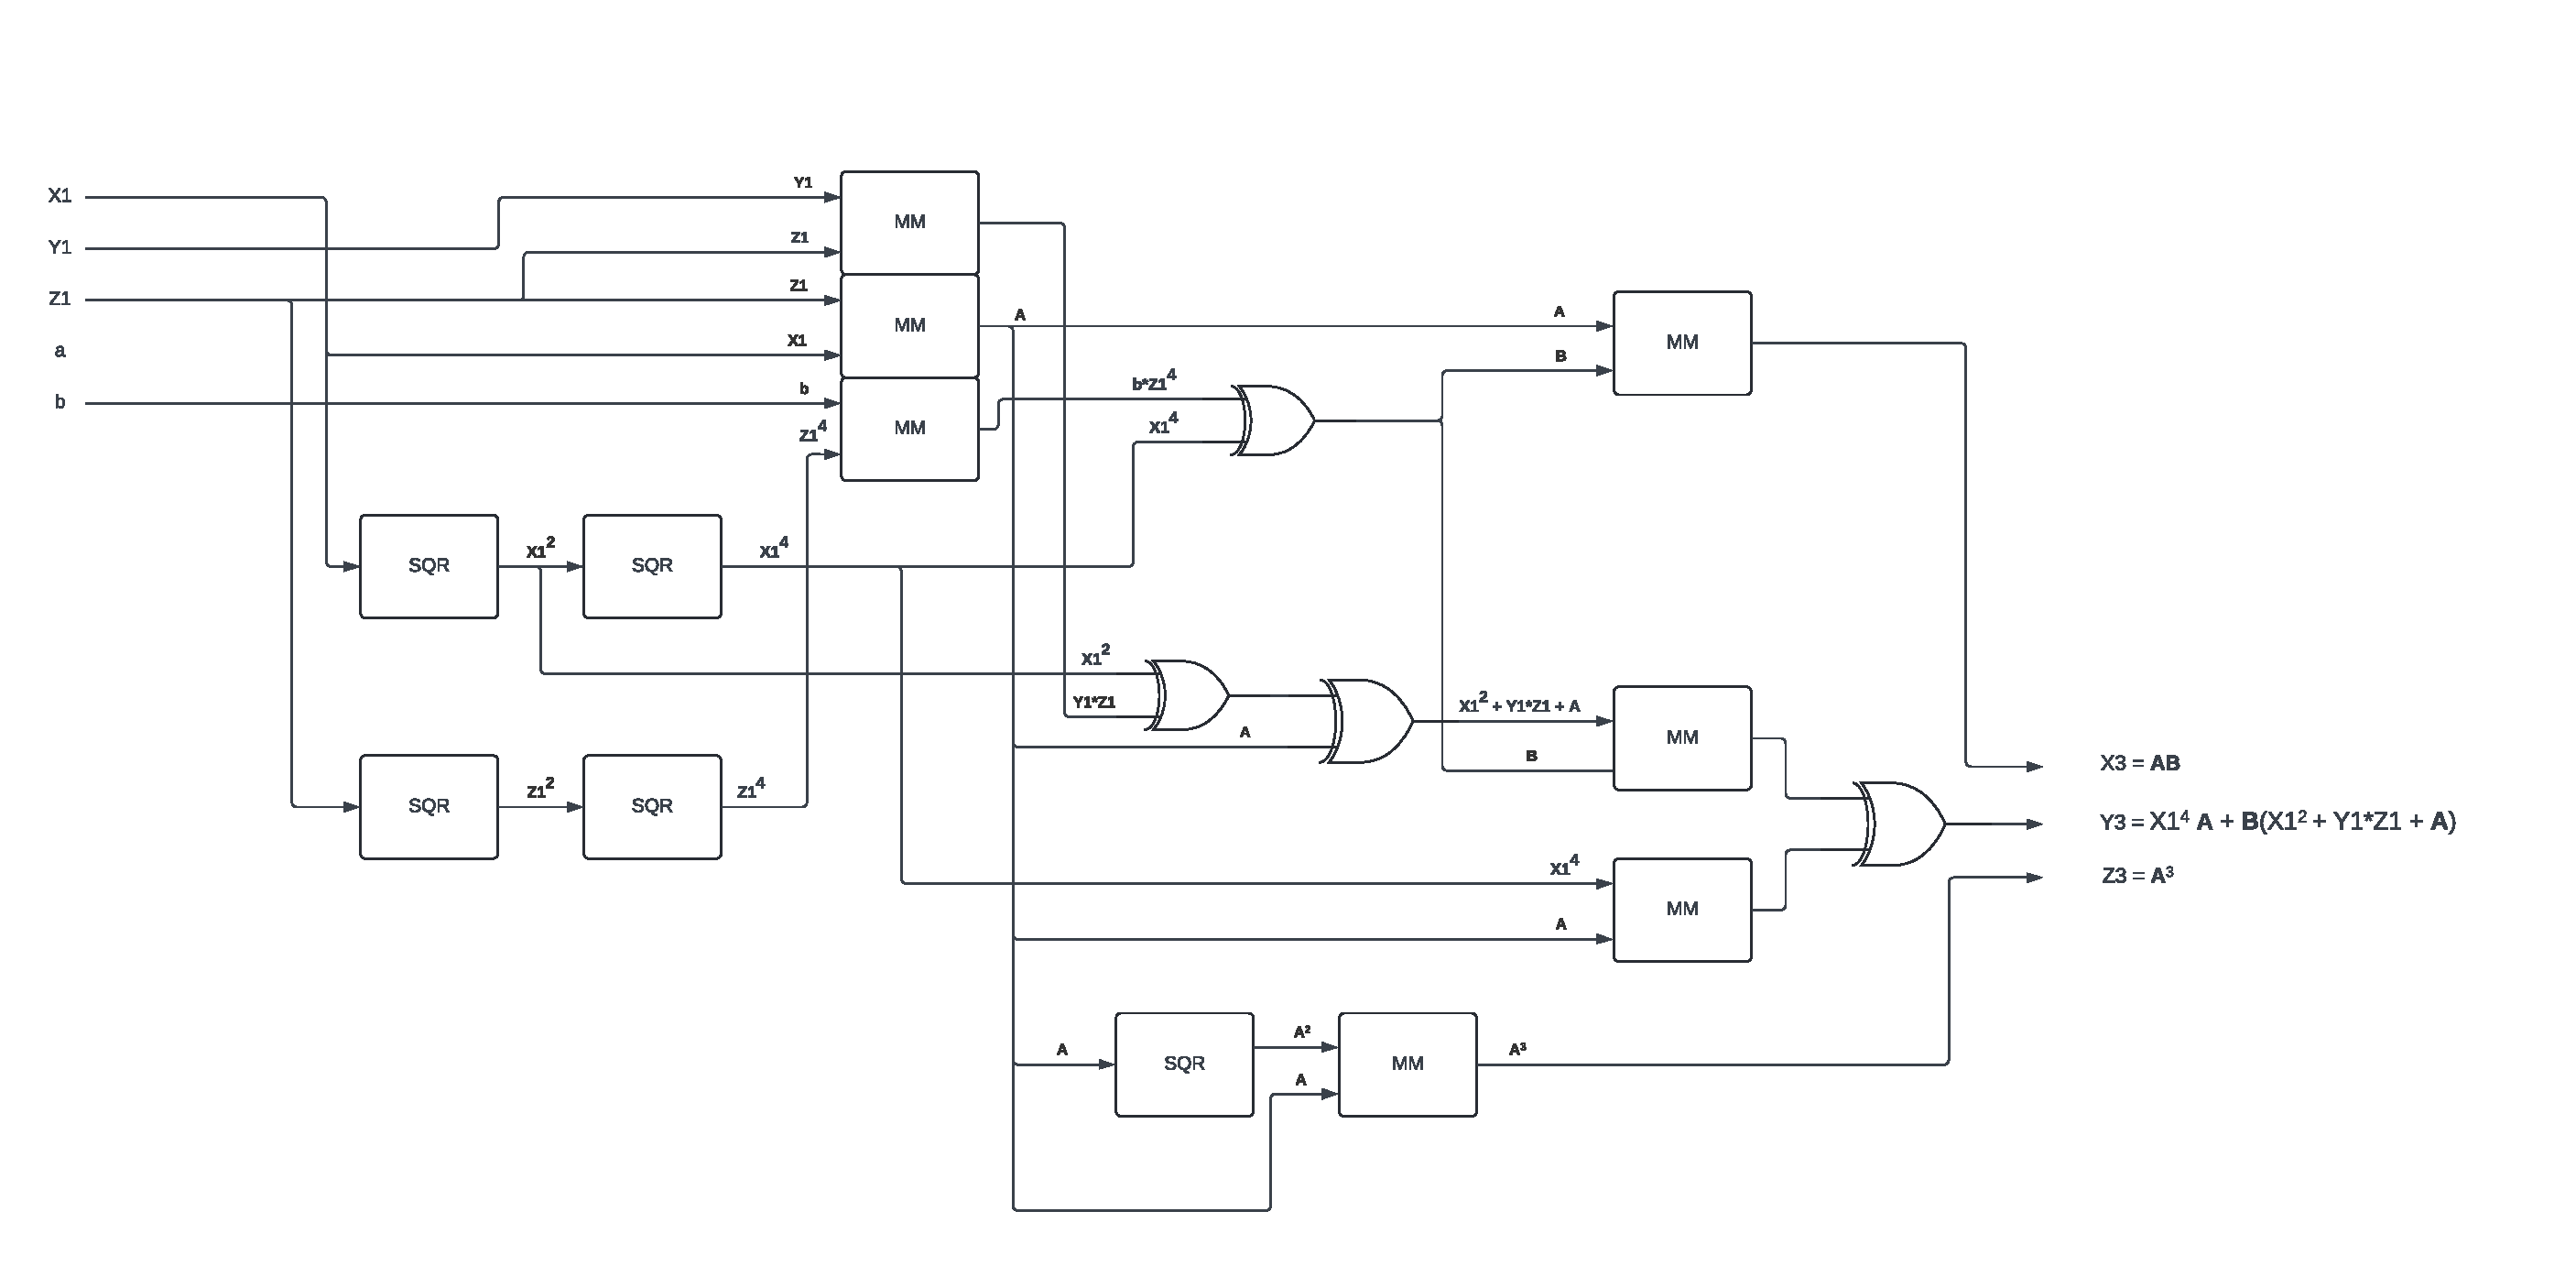
\includegraphics[width=19.5cm]{./images/DATA_FLOW_GRAPH_projective.pdf}
    \caption{Dataflow graph}
    \label{fig:dfg}
  \end{figure}
\end{center}



\subsection{h) Simulation and example demonstrations}
\label{sec:orgb5a8637}
 Demonstrate that your PointDouble() module correctly computes the doubling of the
following affine points:

\begin{verbatim}
cat ./verilog/testbenches/TB_DOUB_PROJ.log
\end{verbatim}


\[
\subsubsection{Results of Point Doubling Projective log}
\begin{lstlisting}[language=Singular]
Time	X1	Y1	Z1	X3	Y3	Z3
10	xxx	xxx	xxx	xxx	xxx	xxx
20	010	001	001	001	110	101
30	010	001	001	001	110	101
40	101	011	001	111	010	100
50	101	011	001	111	010	100
60	011	001	001	100	101	010
70	011	001	001	100	101	010
80	000	001	001	000	001	000
If reached, no errors present in logic.
End of simulation @ 80 ns
\end{lstlisting}
\]






\subsubsection{Defining projective plane}
\label{sec:org8c7b61a}
Pick \(Z_1 = 1\) to keep computations simple. Note that since each coordinate of a point is
in \(\mathbb{F}_8\) , each of \(X_1, Y_1, Z_1\) is a 3-bit vector.

\subsubsection{\(P = (\alpha, 1)\) simulate \(2P\)}
\label{sec:org0bd8ecd}
For affine point \(P = (\alpha, 1)\), simulate \(2P\) on your Verilog Testbench. What is \(2P\)?
\subsubsection{\(P = (\alpha^3, \alpha + 1)\) simulate \(2P\)}
\label{sec:orgb2c67aa}
For affine point \(P = (\alpha^3, \alpha + 1)\), simulate \(2P\) on your Verilog Testbench. What is \(2P\) for
this case?
\subsubsection{Notes:}
\label{sec:org81d4b18}
Note that \((X_1 , Y_1 , Z_1 )\) computed by your circuit is actually \((\frac{X_1}{Z_1}, \frac{Y_1}{Z_1})\) in the affine
space! You can of course check your answer with Singular.
\end{document}